%% -*-TeX-*-
 % ###################################################################
 %  FiPy - a finite volume PDE solver in Python
 % 
 %  FILE: "fipy.tex"
 %                                    created: 4/1/04 {2:58:37 PM} 
 %                                last update: 7/30/04 {9:53:31 PM} 
 %  Author: Jonathan Guyer
 %  E-mail: guyer@nist.gov
 %  Author: Daniel Wheeler
 %  E-mail: daniel.wheeler@nist.gov
 %    mail: NIST
 %     www: http://ctcms.nist.gov
 %  
 % ========================================================================
 % This document was prepared at the National Institute of Standards
 % and Technology by employees of the Federal Government in the course
 % of their official duties.  Pursuant to title 17 Section 105 of the
 % United States Code this document is not subject to copyright
 % protection and is in the public domain.  fipy.tex
 % is an experimental work.  NIST assumes no responsibility whatsoever
 % for its use by other parties, and makes no guarantees, expressed
 % or implied, about its quality, reliability, or any other characteristic.
 % We would appreciate acknowledgement if the document is used.
 % 
 % This document can be redistributed and/or modified freely
 % provided that any derivative works bear some notice that they are
 % derived from it, and any modified versions bear some notice that
 % they have been modified.
 % ========================================================================
 % See the file "license.terms" for information on usage and  redistribution of
 % this file, and for a DISCLAIMER OF ALL WARRANTIES.
 %  
 % ###################################################################
 %%

\documentclass[letterpaper]{book}

\usepackage[text={7in,9.333in}]{geometry}

\usepackage{crop}

\usepackage{alltt, parskip, boxedminipage} % fancyheadings,  
\usepackage{multirow, longtable, makeidx, tocbibind, amssymb} 
\usepackage{amsmath} 

\usepackage{minitoc}
% \setcounter{tocdepth}{0}
\setcounter{parttocdepth}{1}

\usepackage[ascii]{inputenc}

%\usepackage{multirow, longtable, tocbibind, amssymb} % makeidx, 
% \usepackage{fullpage}
%\usepackage[headings]{fullpage}
\makeindex
\usepackage[usenames]{color}
\definecolor{darkblue}{rgb}{0,0.05,0.35}
\definecolor{redish}{rgb}{0.894,0.122,0.122}
\definecolor{bluish}{rgb}{0.216,0.188,0.533}
% \usepackage[dvips, pagebackref, pdftitle={FiPy}, pdfcreator={epydoc 2.1}, bookmarks=true, bookmarksopen=false, pdfpagemode=UseOutlines, colorlinks=true, linkcolor=black, anchorcolor=black, citecolor=black, filecolor=black, menucolor=black, pagecolor=black, urlcolor=darkblue]{hyperref}
\usepackage[urlcolor=blue,linkcolor=blue,bookmarksopen,bookmarksopenlevel=2,pdftex,pagebackref,pdftitle={FiPy}, pdfcreator={epydoc 2.1}, bookmarks=true, bookmarksopen=false, pdfpagemode=UseOutlines,colorlinks=true,plainpages=false,pdfpagelabels]{hyperref}
\usepackage{graphicx}
% \usepackage{memhfixc}
% \usepackage{nameref}

\graphicspath{{../figures/}}

% for reStructuredText
\usepackage{shortvrb}
\usepackage{tabularx}
\setlength{\extrarowheight}{2pt}
\newlength{\admonitionwidth}
\setlength{\admonitionwidth}{0.9\textwidth}
\newlength{\docinfowidth}
\setlength{\docinfowidth}{0.9\textwidth}
\newlength{\locallinewidth}
\newcommand{\optionlistlabel}[1]{\bf #1 \hfill}
\newenvironment{optionlist}[1]
{\begin{list}{}
  {\setlength{\labelwidth}{#1}
   \setlength{\rightmargin}{1cm}
   \setlength{\leftmargin}{\rightmargin}
   \addtolength{\leftmargin}{\labelwidth}
   \addtolength{\leftmargin}{\labelsep}
   \renewcommand{\makelabel}{\optionlistlabel}}
}{\end{list}}
% begin: floats for footnotes tweaking.
\setlength{\floatsep}{0.5em}
\setlength{\textfloatsep}{\fill}
\addtolength{\textfloatsep}{3em}
\renewcommand{\textfraction}{0.5}
\renewcommand{\topfraction}{0.5}
\renewcommand{\bottomfraction}{0.5}
\setcounter{totalnumber}{50}
\setcounter{topnumber}{50}
\setcounter{bottomnumber}{50}
% end floats for footnotes
% some commands, that could be overwritten in the style file.
\newcommand{\rubric}[1]{\subsection*{~\hfill {\it #1} \hfill ~}}
\newcommand{\titlereference}[1]{\textsl{#1}}


\newcommand{\logo}{\rotatebox{4}{\textcolor{redish}{\( \varphi \)}}\kern-.70em\raisebox{-.15em}{\textcolor{bluish}{\( \pi\)}}}
% \newcommand{\logoToo}{\raisebox{-.15em}{\textcolor{bluish}{\(\pi\)}}\kern-.64em\rotatebox{4}{\textcolor{redish}{\( \varphi \)}}}

% commands for various weblinks
%%%%%%%%%%%%%%%%%%%%%%%%%%%%%%%

\newcommand{\FiPy}{\textsf{FiPy}}

\newcommand{\SciPy}{\href{http://www.scipy.org/}{\textsf{SciPy}}}

\newcommand{\PyRex}{\href{http://www.cosc.canterbury.ac.nz/~greg/python/Pyrex/}{\textsf{PyRex}}}

\newcommand{\Python}{\href{http://www.python.org/}{\textsf{Python}}}

\newcommand{\Numeric}{\href{http://www.numpy.org/}{\textsf{Numeric}}}

\newcommand{\NIST}{\href{http://www.nist.gov/}{\textsf{NIST}}}

\newcommand{\CTCMS}{\href{http://www.ctcms.nist.gov/}{\textsf{CTCMS}}}

\newcommand{\MSEL}{\href{http://www.msel.nist.gov/}{\textsf{MSEL}}}

\newcommand{\PyX}{\href{http://pyx.sourceforge.net/}{\textsf{PyX}}}

\newcommand{\PyGist}{\href{http://bonsai.ims.u-tokyo.ac.jp/~mdehoon/software/python/pygist.html}{\textsf{PyGist}}}

\newcommand{\MacOSX}{\href{http://www.apple.com/macosx/}{\textsf{Mac OS X}}}

\newcommand{\Gmsh}{\href{http://www.geuz.org/gmsh/}{\textsf{Gmsh}}}

\newcommand{\weave}{\href{http://www.scipy.org/documentation/weave/}{\textsf{weave}}}

\newcommand{\doctest}{\href{http://www.python.org/doc/current/lib/module-doctest.html}{\textsf{doctest}}}

\newcommand{\unittest}{\href{http://www.python.org/doc/current/lib/module-unittest.html}{\textsf{unittest}}}

%%%%%%%%%%%%%%%%%%%%%%%%%%%%%%%%

% \includeonly{installation}

\makeatletter
\renewcommand*\l@section{\@dottedtocline{1}{1.5em}{3.3em}}
\renewcommand*\l@subsection{\@dottedtocline{2}{3.8em}{4.2em}}
\renewcommand*\l@subsubsection{\@dottedtocline{3}{7.0em}{5.1em}}
\renewcommand*\l@paragraph{\@dottedtocline{4}{10em}{6em}}
\renewcommand*\l@subparagraph{\@dottedtocline{5}{12em}{7em}}

\renewcommand\tableofcontents{%
    \if@twocolumn
      \@restonecoltrue\onecolumn
    \else
      \@restonecolfalse
    \fi
    \chapter*{\contentsname\pdfbookmark[-1]{Contents}{contents}
        \@mkboth{%
           \MakeUppercase\contentsname}{\MakeUppercase\contentsname}}%
    \@starttoc{toc}%
    \if@restonecol\twocolumn\fi
    }

\renewcommand\maketitle{\begin{titlepage}%
\let\footnotesize\small
\let\footnoterule\relax
\let \footnote \thanks
\null\vfil
\vskip 20\p@
\begin{flushright}%
  {\Huge \@title \par}%
  \vskip 3em%
  {\large
   \lineskip .75em%
    \begin{tabular}[t]{r@{}}%
      \@author
    \end{tabular}\par}%
    \vskip 1.5em%
  {\large \@date \par}%       % Set date in \large size.
\end{flushright}\par
\@thanks
\vfil\null
\end{titlepage}%
\setcounter{footnote}{0}%
\global\let\thanks\relax
\global\let\maketitle\relax
\global\let\@thanks\@empty
\global\let\@author\@empty
\global\let\@date\@empty
\global\let\@title\@empty
\global\let\title\relax
\global\let\author\relax
\global\let\date\relax
\global\let\and\relax
}

\makeatother

% \usepackage{layout}


\usepackage{tocvsec2}

\input{version}

\begin{document}

\doparttoc

% \crop[frame,axes]

\frontmatter

% \layout

% \settypeblocksize{9in}{7in}{*}
% \setlrmargins{*}{*}{*}
% \setulmargins{*}{*}{*}

% \settrimmedsize{8.5in}{11in}{*}       % pi/2
% % \settypeblocksize{40\onelineskip}{*}{0.61803}  % golden ratio
% \settypeblocksize{33\onelineskip}{*}{0.61803}  % golden ratio
% \setlength{\trimtop}{0pt}
% \setlength{\trimedge}{\stockwidth}
% \addtolength{\trimedge}{-\paperwidth}
% \addtolength{\trimedge}{-1.5in}
% \setlrmargins{*}{*}{2}
% % \setlrmargins{*}{1in}{*}
% \setulmargins{5\onelineskip}{*}{*}
% \setheadfoot{3\onelineskip}{3\onelineskip}
% \setheaderspaces{\onelineskip}{*}{*}
% \setmarginnotes{17pt}{65pt}{\onelineskip}

% \checkandfixthelayout

% \fixpdflayout

% \setlength{\parindent}{0ex}
\setlength{\fboxrule}{2\fboxrule}
\newlength{\BCL} % base class length, for base trees.

% \pagestyle{Ruled}
\renewcommand{\sectionmark}[1]{\markboth{#1}{}}
\renewcommand{\subsectionmark}[1]{\markright{#1}}

\newenvironment{Ventry}[1]%
  {\begin{list}{}{%
    \renewcommand{\makelabel}[1]{\texttt{##1:}\hfil}%
    \settowidth{\labelwidth}{\texttt{#1:}}%
    \setlength{\leftmargin}{\labelsep}%
    \addtolength{\leftmargin}{\labelwidth}}}%
  {\end{list}}

\newsavebox{\NISTbox}
\sbox{\NISTbox}{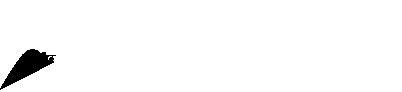
\includegraphics[trim=5 2 5 5,scale=1.5]{NIST_right2line}}
%\newlength{\photoheight}
%\settoheight{\photoheight}{\usebox{\photobox}}
%\newlength{\photowidth}
%\settowidth{\photowidth}{\usebox{\photobox}}

\makeatletter
\newcommand*{\ps@mytitlepage}{%
  \let\@oddhead\@empty
  \renewcommand*{\@oddfoot}{%
  \hfill\parbox[b][0pt]{0pt}{\makebox[0pt][r]{\usebox{\NISTbox}}}}}%\vspace*{-0.5in}}
\makeatother

\makeatletter  
\begin{titlepage}%
\thispagestyle{mytitlepage}
\let\footnotesize\small
\let\footnoterule\relax
\let \footnote \thanks
% \begin{flushleft}
%     \scalebox{10}{\logo}
% \end{flushleft}
% \null\vfil
% \vskip 20\p@
\begin{flushright}%
  \scalebox{10}{\logo}\par
%   \vspace*{\fill}
  \vskip 3em%
  {\Huge FiPy \\
    \huge A Finite Volume PDE Solver Using Python \par}%
  \vskip 3em%
  {\large
   \lineskip .75em%
    \begin{tabular}[t]{r@{}}%
        Daniel Wheeler \\
        Jonathan E. Guyer \\ 
        James A. Warren \\
        \textit{Metallurgy Division} \\
        \textit{Materials Science and Engineering Laboratory}
    \end{tabular}\par}%
    \vskip 1.5em%
  {\large \@date \par}%       % Set date in \large size.
      \vskip 1.5em%
  {\large Version~\Version \par}
% \vfil\null
  \vspace*{\fill}%
%   \raisebox{-5cm}{\fbox{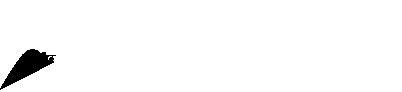
\includegraphics[hiresbb,scale=1.5]{NIST_right2line}}}%
\end{flushright}%
\end{titlepage}%
\makeatother

% \title{
% \scalebox{5}{\logo} \\[2ex]
% \Huge FiPy \\
% A Finite Volume PDE Solver Using Python \\
% }
% 
% \author{Daniel Wheeler, Jonathan E. Guyer \& James A. Warren \\
% Metallurgy Division, Materials Science and Engineering Laboratory\\
% National Institute of Standards and Technology}
% 
% \maketitle

\maxtocdepth{all} 
\tableofcontents
% \faketableofcontents

\mainmatter

\part{Introduction}

\settocdepth{chapter} 
\parttoc

\chapter{Introduction}

\input readme

\section{Aims}

The goal of the |FiPy| framework is to develop a highly customizable
open source code available to the scientific community. |FiPy| allows
users to select and customize modules from within the framework. Those
modules can then be combined with an extremely powerful high level
scripting language allowing the user full control over the solution
algorithm. This 'top down' method of computer programming allows
significant code reuse while accounting for the unique vagaries of
each problem.

The initial development of the framework has been undertaken in the
Center for Theoretical and Computational Materials Science (CTCMS_),
in the Materials Science and Engineering Laboratory (MSEL_) at the
National Institute of Standards and Technology (NIST_). The framework
is known as |FiPy| and is developed at the top level in the Python_
programming language. Python_ enables the integration of low-level
high performance languages such as C and FORTRAN allowing for
efficient optimization. Python_ also has a large repository of free
numerical and scientific software that can be integrated into the
|FiPy| framework. At NIST_, there is a significant ongoing effort to
maximize the efficiency of |FiPy| with the use of third party software
and the judicious use of the C programming language embedded in
standard core modules.

The end goal of |FiPy| is to provide a realistic open source choice
for solving coupled sets of equations. Once an efficient customizable
framework is developed, the end goal will only be achieved with proper
support for the community of users. Many previous scientific computing
projects, although valuable tools, are not adopted by the end users
due to inadequate distribution tools and lack of support. Adequate
support consists of clear documentation, efficient distribution
methods, a code repository, regular code updates (bug fixes) and a
test infrastructure. We aim to address all of these issues.

The aims mentioned above can be summarized as follows:

* Develop core test piece models for various material science problems.
* Develop a highly efficient and customizable code.
* Support the distribution of code to the end users.

\section{Research Background}

The equations that model the evolution of physical, chemical and
biological systems often have a remarkably universal form. Indeed,
partial differential equations (PDEs) have proven necessary to model
complex physical systems and processes that involve variations in both
space and time.  In general, given a variable of interest such as
species concentration, pH or temperature, there exists an evolution
equation of the form
\begin{equation}
  \frac{\partial \phi}{\partial t} = H(\phi, \lambda_i)
  \label{eqn:general-equation}
\end{equation}
where $H$ is a function of $\phi$, other state variables $\lambda_i$,
and higher order derivatives of all of these variables. Examples of
such systems are wide ranging, but include problems that exhibit a
combination of diffusing and reacting species, as well as such diverse
problems as determination of the electric potential in heart tissue,
of fluid flow, stress evolution, and even the Schroedinger equation.

The initial implementation of \FiPy{} has been developed to address
model problems in materials science such as poly-crystals, dendrititic
growth and electrochemical deposition. These applications all contain
various combinations of PDEs with differing forms in conjunction with
other unusual physics (over varying length scales) and unique solution
procedures. The philosophy of \FiPy{} is to enable unique
customization while providing a library of efficient modules for
common objects and data types.

\section{\FiPy{} Philosophy}

It is hard to estimate the future impact of a particular open source
project. However, we believe that the core principles used in the
development of \FiPy{} will enable it to have significant future
growth within the scientific community. The core principles of \FiPy{}
are outlined in some of the following sections.

\subsection{Object Oriented Approach}

\FiPy{} is programmed in an object-oriented manner. The benefit of object
oriented programming mainly lies in encapsulation and
inheritance. Encapsulation allows parts of the code to be separated
into clearly defined independent modules that can be re-applied or
extended in new ways. Inheritance allows code to be reused and new
capabilities to be added without altering the original code. These are
extremely powerful techniques.

\subsection{Test Based Development}

\FiPy{} has been developed with a large number of test cases. These test
cases operate on two levels. The lower level tests operate on the core
modules at the individual method level. Thus every method within the
core installation has a test case. The high level test cases operate
in conjunction with example test piece solutions and test global
solution algorithms and the interaction of various modules. Thus at
any stage in code development the test cases can be executed and
errors can be identified.

A test base is essential for the adoption of the code by new users and
developers. Many numerical codes do not have test bases available with
the code. This is a severe drawback in any prospective development
making it difficult to alter the code without the reassurance that any
code breakages will be clearly demonstrated with a broken test case. A
test base also aids dissemination of the code by providing simple
examples and knowledge of whether the code is working on a particular
computer environment.

\Python{} has modules (\doctest{}, \unittest{}) that automate the testing procedure.

\subsection{Documentation}

FiPY has been developed with a continuously updated manual. The manual
contains introductory material, installation procedures and
explanation of numerical algorithms. The manual also contains an
automated description of each module and method. The automated
description is derived from comments in the source code. Thus the
manual will stay current as the code develops and encourage developers
to comment the code. The same automated method is used to build
descriptions of core examples making it each for a prospective user to
understand and start using the code.

Many numerical codes do not have adequate documentation.

\subsection{Numerical Approach}

The solution algorithms given in the \FiPy{} examples involve combining
sets of PDEs while tracking an interface where the parameters of the
problem change rapidly. The Phase Field Method (PFM) and the Level Set
Method (LSM) are specialized techniques to handle the solution of
PDEs in conjunction with a deforming interface. The combination of
these methods within one code is novel and useful for academic as well
as practical comparison of both methods. Both methods are not new but
are still undergoing constant development.

\FiPy{} uses the well-known Finite Volume Method (FVM) to reduce the
model equations to a form tractable to linear solvers.

In general, both the LSM and PFM methods do not appear with standard
FV solvers, usually the more standard Volume Of Fluid Method (VOFM) is
used as an interface-tracking algorithm. Generally, VOFM is used for
very different applications to the LSM and PFM.

\subsection{Distribution}

Clear distribution techniques and easy installation are required for
prospective users to begin using the code. Two prospective methods are
planned for code distribution. The first method is simply creating
stable archive releases that users can unpack. The second method is to
create a code repository where users can update to the latest unstable
version of the code. This is useful to allow users access to the
latest bug fixes. Also having a central code repository allows more
developers to join the main project or select parts of the project.

Most numerical software is not distributed via a code repository and
thus makes obtaining the latest version of the software and bug fixes
difficult.

\subsection{Open Source}

In recent years there has been a movement towards more open source
unrestrictive licenses especially within the scientific community. The
\FiPy{} framework will be written with an open source license allowing
users to develop with complete access to the source code and then
either contribute back to the main source repository or freely
distribute their new adapted version. Many members of the scientific
community prefer to use an open source license due to the unrestricted
access and ability to develop extensible codes. Specifically, the
restrictions of non-open source licenses involve an inability to
redistribute code, a lack of access to source code and the expense of
maintaining licenses. Redistribution of code not only allows tools to
be shared but also promotes communication of ideas. Access to source
code is essential for developers and users to understand the function
of a code and allow bugs to be fixed.

\subsection{Pair Programming}

\href{http://www.extremeprogramming.org/rules/pair.html}{Pair programming}
is a good way to develop computer code.

\subsection{\Python{} Programming Language}

\Python{} combines remarkable power with very clear syntax. It is
freely usable and distributable, even for commercial use. \Python{} is
an example of an interpreted scripting language. Scripting languages
are seen as distinctive from compiled lower level languages such as C
or FORTRAN. Such lower level languages are commonly used for numerical
codes due to their increased efficiency over scripting languages. This
makes \Python{} an unusual choice for the bases of a numerical
framework.

Codes, programmed exclusively in C or FORTRAN, are often hard to
readapt to new application areas mainly due to the inability to allow
developers access at various levels of the code. In general, such
codes use a distinctive scripting language written for the code at
hand allowing users to vary parameter values and switch between
different internal solution algorithms. Such exclusive scripting
languages can often be difficult to write and must be an integral part
of the design of the numerical code and cannot easily account for the
various ways a prospective user may wish to use the code.

Thus \FiPy{}, rather than taking the approach of writing the fast
numerical code first and then dealing with the issue of user
interaction, initially implements most modules in the \Python{}
scripting language and only translates to C those parts of the code
that prove inefficient. This leads to most top-level structures being
written in \Python{} allowing easy to understand implementation and
modification. The choice of \Python{} is in part due to the easy
integration of C either as separate modules or encapsulated in
\Python{} functions as well as the ability to directly translate from
\Python{} to C (\PyRex{}). This low-level integration has resulted
in a number of freely available efficient numerical modules (\SciPy{},
\Numeric{}) for \Python{} some of which are utilized in the \FiPy{}
framework.

\section{Contributions}

\section{Sourceforgre}

Mailing lists, bug tracking, 

\section{Outstanding Issues}

\subsection{Efficiency}

\subsection{Memory Usage}

\chapter{Installation}

\inputencoding{latin1}

\input installation

\inputencoding{ascii}

This chapter describes the numerical methods used to solve equations
in the \FiPy{} programming environment. \FiPy{} uses the finite volume
method (FVM) to solve coupled sets of partial differential equations
(PDEs). For a good introduction to the FVM see Nick Croft's PhD
thesis~\cite{croftphd}, Patanker~\cite{patanker} or Versteek and
Malalasekera~\cite{versteegMalalasekera}.

Essentially, the FVM consists of dividing the solution domain into
discrete finite volumes over which the state variables are
approximated with linear or higher order interpolations. The
derivatives in each term of the equation are satisfied with simple
approximate interpolations in a process known as discretization. The
(FVM) is a popular discretization technique employed to solve coupled
PDEs used in many application areas (\emph{e.g.} Fluid Dynamics).

The FVM can be thought of as a subset of the Finite Element Method
(FEM) as the Finite Difference Method (FDM) is a subset of the FVM. A
system of equations fully equivalent to the FVM can be obtained with
the FEM using as weighting functions the characteristic functions of
FV cells, i.e., functions equal to unity~\cite{mattiussi:1997}. Analogously,
the the discretization of equations with the FVM reduces to the FDM on
Cartesian grids.

\input numerical/equation
\input numerical/discret
\input numerical/scheme




\settocdepth{all} 

\part{Examples}

\settocdepth{chapter} 
\parttoc

\chapter{Diffusion Examples}

\input{examples/latex/examples.diffusion.steadyState.mesh1D.input-module}
\newpage
\input{examples/latex/examples.diffusion.steadyState.mesh1D.tri2Dinput-module}
\newpage
\input{examples/latex/examples.diffusion.steadyState.mesh20x20.input-module}
\newpage
\input{examples/latex/examples.diffusion.steadyState.mesh50x50.input-module}
\newpage
\input{examples/latex/examples.diffusion.explicit.mesh10.input-module}
\newpage
\input{examples/latex/examples.diffusion.explicit.mesh50.input-module}
\newpage
\input{examples/latex/examples.diffusion.variable.mesh2x1.input-module}
\newpage
\input{examples/latex/examples.diffusion.variable.mesh10x1.input-module}
\newpage
\input{examples/latex/examples.diffusion.variable.mesh50x1.input-module}
\newpage
\input{examples/latex/examples.diffusion.nthOrder.input2ndOrder1D-module}
\newpage
\input{examples/latex/examples.diffusion.nthOrder.input4thOrder1D-module}
\newpage

\chapter{Convection Examples}

\input{examples/latex/examples.convection.exponential1D.input-module}
\newpage
\input{examples/latex/examples.convection.exponential1DBack.input-module}
\newpage
\input{examples/latex/examples.convection.exponential1DSource.input-module}
\newpage
\input{examples/latex/examples.convection.exponential2D.input-module}
\newpage
\input{examples/latex/examples.convection.powerLaw1D.input-module}
\newpage

\chapter{Phase Field Examples}

\input{examples/latex/examples.phase.anisotropy.input-module}
\newpage
\input{examples/latex/examples.phase.impingement.mesh40x1.input-module}
\newpage
\input{examples/latex/examples.phase.impingement.mesh20x20.input-module}
\newpage
\input{examples/latex/examples.phase.impingement.restart.input-module}
\newpage
\input{examples/latex/examples.phase.missOrientation.circle.input-module}
\newpage
\input{examples/latex/examples.phase.missOrientation.mesh1D.input-module}
\newpage
\input{examples/latex/examples.phase.missOrientation.modCircle.input-module}
\newpage
\input{examples/latex/examples.phase.symmetry.input-module}
\newpage

\chapter{Level Set Examples}

\input{examples/latex/examples.levelSet.distanceFunction.oneD.input-module}
\newpage
\input{examples/latex/examples.levelSet.distanceFunction.square.input-module}
\newpage
\input{examples/latex/examples.levelSet.distanceFunction.circle.input-module}
\newpage
\input{examples/latex/examples.levelSet.distanceFunction.interior.input-module}
\newpage
\input{examples/latex/examples.levelSet.advection.mesh1D.input-module}
\newpage
\input{examples/latex/examples.levelSet.advection.circle.input-module}
\newpage

\chapter{Electrochemistry Phase Field Examples}

\input{examples/latex/examples.elphf.input1Dphase-module}
\newpage
\input{examples/latex/examples.elphf.input1D-module}
\newpage
\input{examples/latex/examples.elphf.input1Ddimensional-module}
\newpage
\input{examples/latex/examples.elphf.input2D-module}
\newpage
\input{examples/latex/examples.elphf.input2Dcorner-module}
\newpage
\input{examples/latex/examples.elphf.input1DpoissonAllCharge-module}
\newpage
\input{examples/latex/examples.elphf.input1DpoissonLeftCharge-module}
\newpage
\input{examples/latex/examples.elphf.input1DpoissonRightCharge-module}
\newpage
\input{examples/latex/examples.elphf.input1DphaseBinary-module}
\newpage
\input{examples/latex/examples.elphf.input1DphaseQuaternary-module}
\newpage
\input{examples/latex/examples.elphf.input1DphaseTernAndElectrons-module}
\newpage

\chapter{Cahn-Hilliard Examples}

\input{examples/latex/examples.cahnHilliard.cahnHilliardTanh1D-module}
\newpage

\settocdepth{all} 

% \include{examples}
% 
% \include{theory}
% 
% \include{code}
 
\appendix

\part{APIs}

\settocdepth{chapter} 

\parttoc

\input api

\settocdepth{all} 

\backmatter

%%%%%%%%%%%%%%%%%%%%%%%%%%%%%%%%%%%%%%%%%%%%%%%%%%%%%%%%%%%%%%%%%%%%%%%%%%%
%%                                 Index                                 %%
%%%%%%%%%%%%%%%%%%%%%%%%%%%%%%%%%%%%%%%%%%%%%%%%%%%%%%%%%%%%%%%%%%%%%%%%%%%

% \pdfbookmark[-1]{Index}{index}
\printindex


\end{document}
